\documentclass[ignorenonframetext,t]{beamer}
\setbeamertemplate{caption}[numbered]
\setbeamertemplate{caption label separator}{: }
\setbeamercolor{caption name}{fg=normal text.fg}
\beamertemplatenavigationsymbolsempty
\usepackage{lmodern}
\usepackage{amssymb,amsmath}
\usepackage{ifxetex,ifluatex}
\usepackage{fixltx2e} % provides \textsubscript
\ifnum 0\ifxetex 1\fi\ifluatex 1\fi=0 % if pdftex
  \usepackage[T1]{fontenc}
  \usepackage[utf8]{inputenc}
\else % if luatex or xelatex
  \ifxetex
    \usepackage{mathspec}
  \else
    \usepackage{fontspec}
  \fi
  \defaultfontfeatures{Ligatures=TeX,Scale=MatchLowercase}
\fi
\usecolortheme{spruce}
\usefonttheme{serif}
% use upquote if available, for straight quotes in verbatim environments
\IfFileExists{upquote.sty}{\usepackage{upquote}}{}
% use microtype if available
\IfFileExists{microtype.sty}{%
\usepackage{microtype}
\UseMicrotypeSet[protrusion]{basicmath} % disable protrusion for tt fonts
}{}
\newif\ifbibliography
\hypersetup{
            pdftitle={Week 6: Graphical Data Exploriation},
            colorlinks=true,
            linkcolor=Maroon,
            citecolor=Blue,
            urlcolor=blue,
            breaklinks=true}
\urlstyle{same}  % don't use monospace font for urls
\usepackage{longtable,booktabs}
\usepackage{caption}
% These lines are needed to make table captions work with longtable:
\makeatletter
\def\fnum@table{\tablename~\thetable}
\makeatother

% Prevent slide breaks in the middle of a paragraph:
\widowpenalties 1 10000
\raggedbottom

\AtBeginPart{
  \let\insertpartnumber\relax
  \let\partname\relax
  \frame{\partpage}
}
\AtBeginSection{
  \ifbibliography
  \else
    \let\insertsectionnumber\relax
    \let\sectionname\relax
    \frame{\sectionpage}
  \fi
}
\AtBeginSubsection{
  \let\insertsubsectionnumber\relax
  \let\subsectionname\relax
  \frame{\subsectionpage}
}

\setlength{\parindent}{0pt}
\setlength{\parskip}{6pt plus 2pt minus 1pt}
\setlength{\emergencystretch}{3em}  % prevent overfull lines
\providecommand{\tightlist}{%
  \setlength{\itemsep}{0pt}\setlength{\parskip}{0pt}}
\setcounter{secnumdepth}{0}
\usepackage{multicol}
\usepackage{tikz}
\usepackage{tikzpagenodes}
\definecolor{grn}{rgb}{0.0, 0.2, 0.0}
\usepackage{tabto}
\usepackage{verbatim}
\usepackage{amsmath}
\usepackage{mathtools}
\usepackage{graphicx}
\definecolor{OG}{RGB}{0,64,8}
\definecolor{LG}{RGB}{0,102,51}
\definecolor{myRed}{RGB}{228,26,28}
\definecolor{myBlue}{RGB}{55,126,184}
\definecolor{myGreen}{RGB}{77,175,74}
\definecolor{myPurple}{RGB}{152,78,163}
\setbeamercolor{itemize item}{fg=white!0!LG}
\setbeamercolor{enumerate item}{fg=white!0!LG}
\setbeamercolor{enumerate subitem}{fg=white!70!LG}
\setbeamercolor{itemize subitem}{fg=white!70!LG}
\setbeamercolor{itemize subsubitem}{fg=white!70!LG}
\setbeamercolor{navigation symbols}{fg=white!70!LG, bg=white!70!LG}
\usepackage{inputenc}
\usepackage{booktabs}
\usepackage{caption}
\usetikzlibrary{patterns,arrows,decorations.pathreplacing}

\title{Week 6: Graphical Data Exploriation}
\subtitle{Session 2}
\date{Spring 2020}

\begin{document}
\frame{\titlepage}

\begin{frame}[fragile]{iClicker Question \textcolor{blue}{1}}

Which of the following should I use to read the file \texttt{mydata.csv}
into a data frame called \texttt{dat} in R?

\begin{enumerate}[A]
\item \texttt{dat = read.csv(mydata.csv)}
\item \texttt{read.csv(mydata.csv)}
\item \texttt{dat = read.csv("mydata.csv")}
\item \texttt{read.csv(mydata.csv, row.names = 1)}
\item \texttt{read.csv("mydata.csv")}
\end{enumerate}

\vfill

\begin{tikzpicture}[remember picture,overlay]
\node[xshift=-2cm,yshift=1cm] at (current page.south east)
{
\includegraphics[height=0.25in]{../slide_images/iClicker_logo.png}};
\end{tikzpicture}

\end{frame}

\begin{frame}[fragile]{iClicker Question \textcolor{blue}{2}}

Which of the following lines of code will make a scatterplot with a
custom \textbf{title}?

\begin{verbatim}
##      length     width mass
## 1 0.7209039 2.8777226   37
## 2 0.8757732 1.6052823   29
## 3 0.7609823 0.4713699   19
\end{verbatim}

\begin{enumerate}[A]
\item \texttt{plot(dat\$mass, dat\$length, col = 3)}
\item \texttt{plot(dat\$mass, dat\$length, type = "l")}
\item \texttt{plot(dat\$length, dat\$mass, type = "p")}
\item \texttt{plot(dat\$mass, dat\$length, main = "data plot")}
\item \texttt{plot(dat\$length, dat\$mass)}
\end{enumerate}

\vfill

\begin{tikzpicture}[remember picture,overlay]
\node[xshift=-2cm,yshift=1cm] at (current page.south east)
{
\includegraphics[height=0.25in]{../slide_images/iClicker_logo.png}};
\end{tikzpicture}

\end{frame}

\begin{frame}{iClicker Question \textcolor{blue}{3}}

Which is the best location for me to type my R code for in-class and
individual activities?

\begin{enumerate}[A]
\item A text file in Word or another word processor
\item The RStudio console pane
\item The RStudio code editor pane
\item The RStudio Environment pane
\end{enumerate}

\vfill

\begin{tikzpicture}[remember picture,overlay]
\node[xshift=-2cm,yshift=1cm] at (current page.south east)
{
\includegraphics[height=0.25in]{iClicker_logo.png}};
\end{tikzpicture}

\end{frame}

\begin{frame}{Announcements}

\end{frame}

\begin{frame}{Follow-up questions from the Chapter 5 homework}

Error in Tuesday's title slide is now fixed. You can re-download the
correct version on Moodle.

Week 5 reading assignment question \# 1:

``What is the difference between parametric and a non-parametric
distribution?''

\begin{itemize}
\item
  The book's explanation of \emph{parametric distribution} is slightly
  misleading. The reading characterizes the Normal distribution as a
  parametric distribution, however there are many \emph{parametric
  distributions}. I like to use the term \emph{theoretical
  distributions} when I'm describing \emph{parametric distributions} to
  emphasize that they are precisely mathematically defined. The behavior
  of \emph{parametric distributions} is governed by 1 or more
  \emph{parameters} in the probability functions.
\item
  What is a \textbf{non-parametric distribution}?
\end{itemize}

Question 3: ``In R, what would be returned if you compute the mean value
of a vector containing the following values: 4, 9, 2, 13, NA, 9? Please
describe your methods.''"

\begin{itemize}
\tightlist
\item
  Question from me: Is there a benefit to having mean() fail when you
  pass an NA?
\end{itemize}

\end{frame}

\begin{frame}{For Today}

Are there any general questions about data exploration, numeric or
graphical?

Short lecture

Group activity: graphical data exploration part 2 - rarefaction data.

We'll start to use \emph{inference} in the coming weeks!

\end{frame}

\begin{frame}{Some graphics pointers}

In summary, graphs are a useful data visualization tool

\begin{itemize}
\tightlist
\item
  summarizing
\item
  understanding
\item
  describing
\item
  presenting/communicating
\end{itemize}

\end{frame}

\begin{frame}{Some graphics pointers}

In summary, graphs are a useful data visualization tool

\begin{itemize}
\tightlist
\item
  summarizing
\item
  understanding
\item
  describing
\item
  presenting/communicating
\end{itemize}

\textbf{BUT} we must label the well or they are useless!

\begin{itemize}
\tightlist
\item
  label both axes
\item
  provide a main title for your graph
\item
  avoid clutter
\item
  make it readable
\item
  \emph{I expect graphs to be propery labeled from now on}!
\end{itemize}

\end{frame}

\begin{frame}{Some graphics pointers}

In summary, graphs are a useful data visualization tool

\vspace{1cm}

\begin{longtable}[]{@{}ll@{}}
\toprule
Purpose & Graph Type\tabularnewline
\midrule
\endhead
Illustrating \emph{distribution} & Histogram, Density
plot\tabularnewline
& Box(-whisker) plot\tabularnewline
Illustrating \emph{differences} & Bar chart, Box plot\tabularnewline
Illustrating \emph{correlations} & Scatter plot\tabularnewline
Illustrating \emph{associations} & Pie chart, Bar chart\tabularnewline
Illustrating \emph{sample size} & Line plot of running
avg\tabularnewline
\bottomrule
\end{longtable}

\end{frame}

\begin{frame}{Beyond graphs, Towards statistics}

\begin{itemize}
\item
  Graphs are powerful tools that provide insight and understanding of
  the patterns and relationships in the data.
\item
  Don't give us the answer though:

  \begin{itemize}
  \tightlist
  \item
    are differences \emph{significant}?
  \item
    are associations \emph{significatnt}?
  \end{itemize}
\end{itemize}

\begin{tikzpicture}[remember picture,overlay]
\node[yshift=3cm] at (current page.south)
{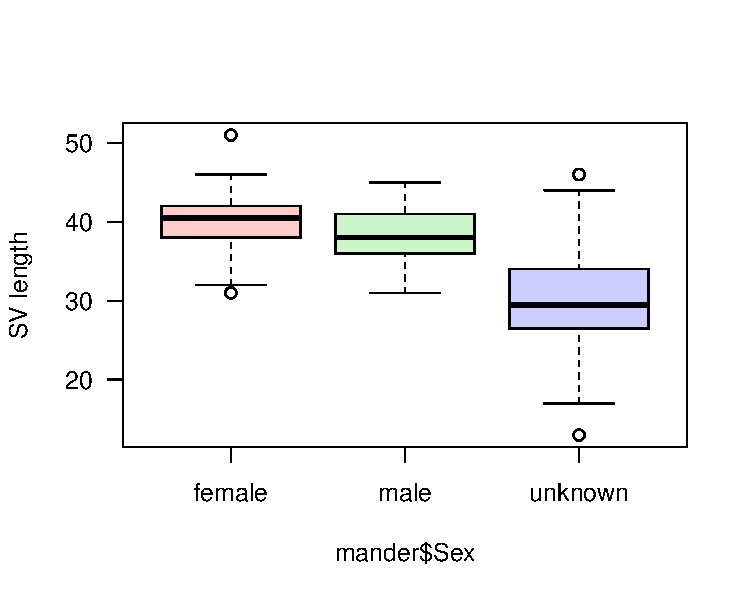
\includegraphics[height=2in]{C:/Users/michaelnelso/git/NRC290B/slides/slide_images/salbox.pdf}};
\end{tikzpicture}

\end{frame}

\begin{frame}{Beyond graphs, Towards statistics}

\begin{itemize}
\item
  Graphs are powerful tools that provide insight and understanding of
  the patterns and relationships in the data.
\item
  Don't give us the answer though:

  \begin{itemize}
  \tightlist
  \item
    are differences \emph{significant}?
  \item
    are associations \emph{significatnt}?
  \end{itemize}
\end{itemize}

\begin{tikzpicture}[remember picture,overlay]
\node[yshift=3cm] at (current page.south)
{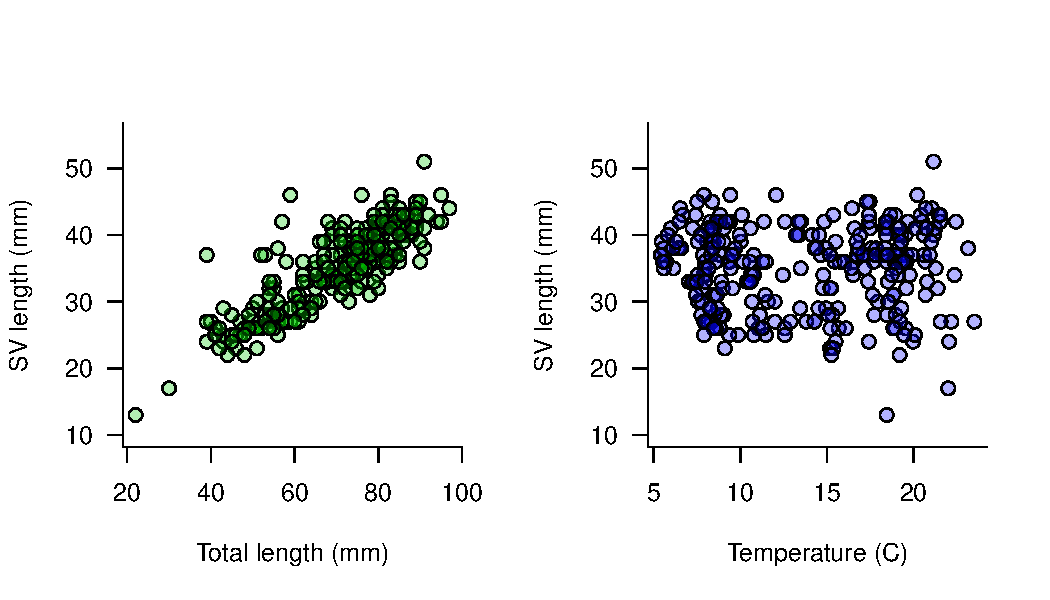
\includegraphics[height=2in]{C:/Users/michaelnelso/git/NRC290B/slides/slide_images/salscatter.pdf}};
\end{tikzpicture}

\end{frame}

\begin{frame}{Beyond graphs, Towards statistics}

\begin{itemize}
\item
  Graphs are powerful tools that provide insight and understanding of
  the patterns and relationships in the data.
\item
  Don't give us the answer though:

  \begin{itemize}
  \tightlist
  \item
    are differences \emph{significant}?
  \item
    are associations \emph{significatnt}?
  \end{itemize}
\item
  Statistics is the tool we use to formally answer these questions!

  \begin{itemize}
  \tightlist
  \item
    the differences \emph{are}/\emph{are not} significant!
  \item
    are associations \emph{are}/\emph{are not} significant!
  \end{itemize}
\end{itemize}

\end{frame}

\begin{frame}{Group graphical activityf}

\end{frame}

\end{document}
